\documentclass[12pt,a4paper]{article}
\usepackage[legalpaper, portrait, margin=2cm]{geometry}
\usepackage[portuguese]{babel}
\usepackage[utf8]{inputenc}
\usepackage{amsmath}
\usepackage{amssymb}
\usepackage{fancyhdr}
\usepackage{graphicx}
\usepackage{hyperref}
\usepackage{indentfirst}
\usepackage{listings}
\usepackage{wrapfig}
\usepackage{xcolor}

\graphicspath{ {./} }
\hypersetup{
  colorlinks=true,
  linkcolor=blue,
  filecolor=magenta,
  urlcolor=blue,
  citecolor=blue,
  pdftitle={Exercício 9 - Projeto Computacional PE 2022/2023 LEIC-A},
  pdfpagemode=FullScreen,
}

\pagenumbering{gobble}
\pagestyle{fancy}
\fancyhf{}
\rhead{Grupo \textbf{11}}
\lhead{Exercício 9 - Projeto Computacional PE 2022/2023 LEIC-A}
\cfoot{Gonçalo Bárias (103124), Raquel Braunschweig (102624) e Vasco Paisana (102533)}

\renewcommand{\footrulewidth}{0.2pt}

\renewcommand{\labelitemii}{$\circ$}
\renewcommand{\labelitemiii}{$\diamond$}

\makeatletter
\newcommand{\srcsize}{\@setfontsize{\srcsize}{8.6pt}{8.6pt}}
\makeatother

\definecolor{codegreen}{rgb}{0,0.6,0}
\definecolor{codegray}{rgb}{0.3,0.3,0.3}
\definecolor{codepurple}{rgb}{0.58,0,0.82}

\lstdefinestyle{mystyle}{
  commentstyle=\color{codegreen},
  numberstyle=\tiny\color{codegray},
  % keywordstyle=\color{magenta},
  % stringstyle=\color{codepurple},
  basicstyle=\ttfamily\srcsize,
  breakatwhitespace=false,
  breaklines=true,
  captionpos=b,
  keepspaces=true,
  numbers=left,
  numbersep=5pt,
  showspaces=false,
  showstringspaces=false,
  showtabs=false,
  tabsize=2
}
\lstset{style=mystyle}

\begin{document}

% Introdução sobre o exercício em questão
Consideremos que foi fixada uma semente igual a \texttt{1166}.
O objetivo deste exercício é o de gerar \texttt{2500} amostras de tamanho $n$, para cada $ n \in \{30, 50, 100, 200, 300, 500, 1000\}$, de uma distribuição de Bernoulli com parâmetro igual a \texttt{0.5}.
De seguida, usar dois métodos distintos que calculam intervalos de confiança de aproximação para o parâmetro mencionado, o que permite obter a diferença entre as amplitudes desses intervalos.
Por fim, calcular a média das \texttt{2500} diferenças para cada $n$.
Para tal, recorreu-se ao seguinte trecho de código em \texttt{R}:

\quad

% Código em R para resolver o exercício
\begin{lstlisting}[language=R]
library("ggplot2")
library("Rlab")

SEED <- 1166
SAMPLE_COUNT <- 2500
BERNOULLI_P <- 0.5
CONF_LEVEL <- 0.97
N <- c(30, 50, 100, 200, 300, 500, 1000)
set.seed(SEED)

method_1 <- function(samples, conf_level) {
    len <- length(samples)
    mean <- mean(samples)
    z <- qnorm((1 + conf_level) / 2)
    sols <- polyroot(c(mean**2, -2 * mean - z**2 / len, 1 + z**2 / len))
    return(abs(sols[2] - sols[1]))
}

method_2 <- function(samples, conf_level) {
    len <- length(samples)
    mean <- mean(samples)
    upper <- mean + qnorm(1 - (1 - conf_level) / 2) * sqrt(mean * (1 - mean) / len)
    lower <- mean - qnorm(1 - (1 - conf_level) / 2) * sqrt(mean * (1 - mean) / len)
    return(abs(upper - lower))
}

df <- data.frame()
for (n in N) {
    method_diffs <- c()
    for (i in 1:SAMPLE_COUNT) {
        samples <- rbern(n, BERNOULLI_P)
        diff <- method_2(samples, CONF_LEVEL) - method_1(samples, CONF_LEVEL)
        method_diffs <- append(method_diffs, diff)
    }
    mean_diffs <- mean(method_diffs)
    df <- rbind(df, data.frame(n = n, difference = mean_diffs))
}

ggplot(df, aes(x = n, y = difference)) +
  geom_line(color = "#e76f51") +
  geom_point(color = "#e76f51") +
  xlab("Dimensão da Amostra") +
  ylab("Variação das Diferenças Médias") +
  labs(title = "Relação entre Variação das Diferenças Médias e Dimensão da Amostra",
    subtitle = sprintf("semente = %d | k = %d | p = %.2f | γ = %.2f",
      SEED, SAMPLE_COUNT, BERNOULLI_P, CONF_LEVEL))
\end{lstlisting}

\quad

% Gráfico para resolver o exercício
\setlength\intextsep{0pt}
\begin{wrapfigure}{r}{0.59\textwidth}
  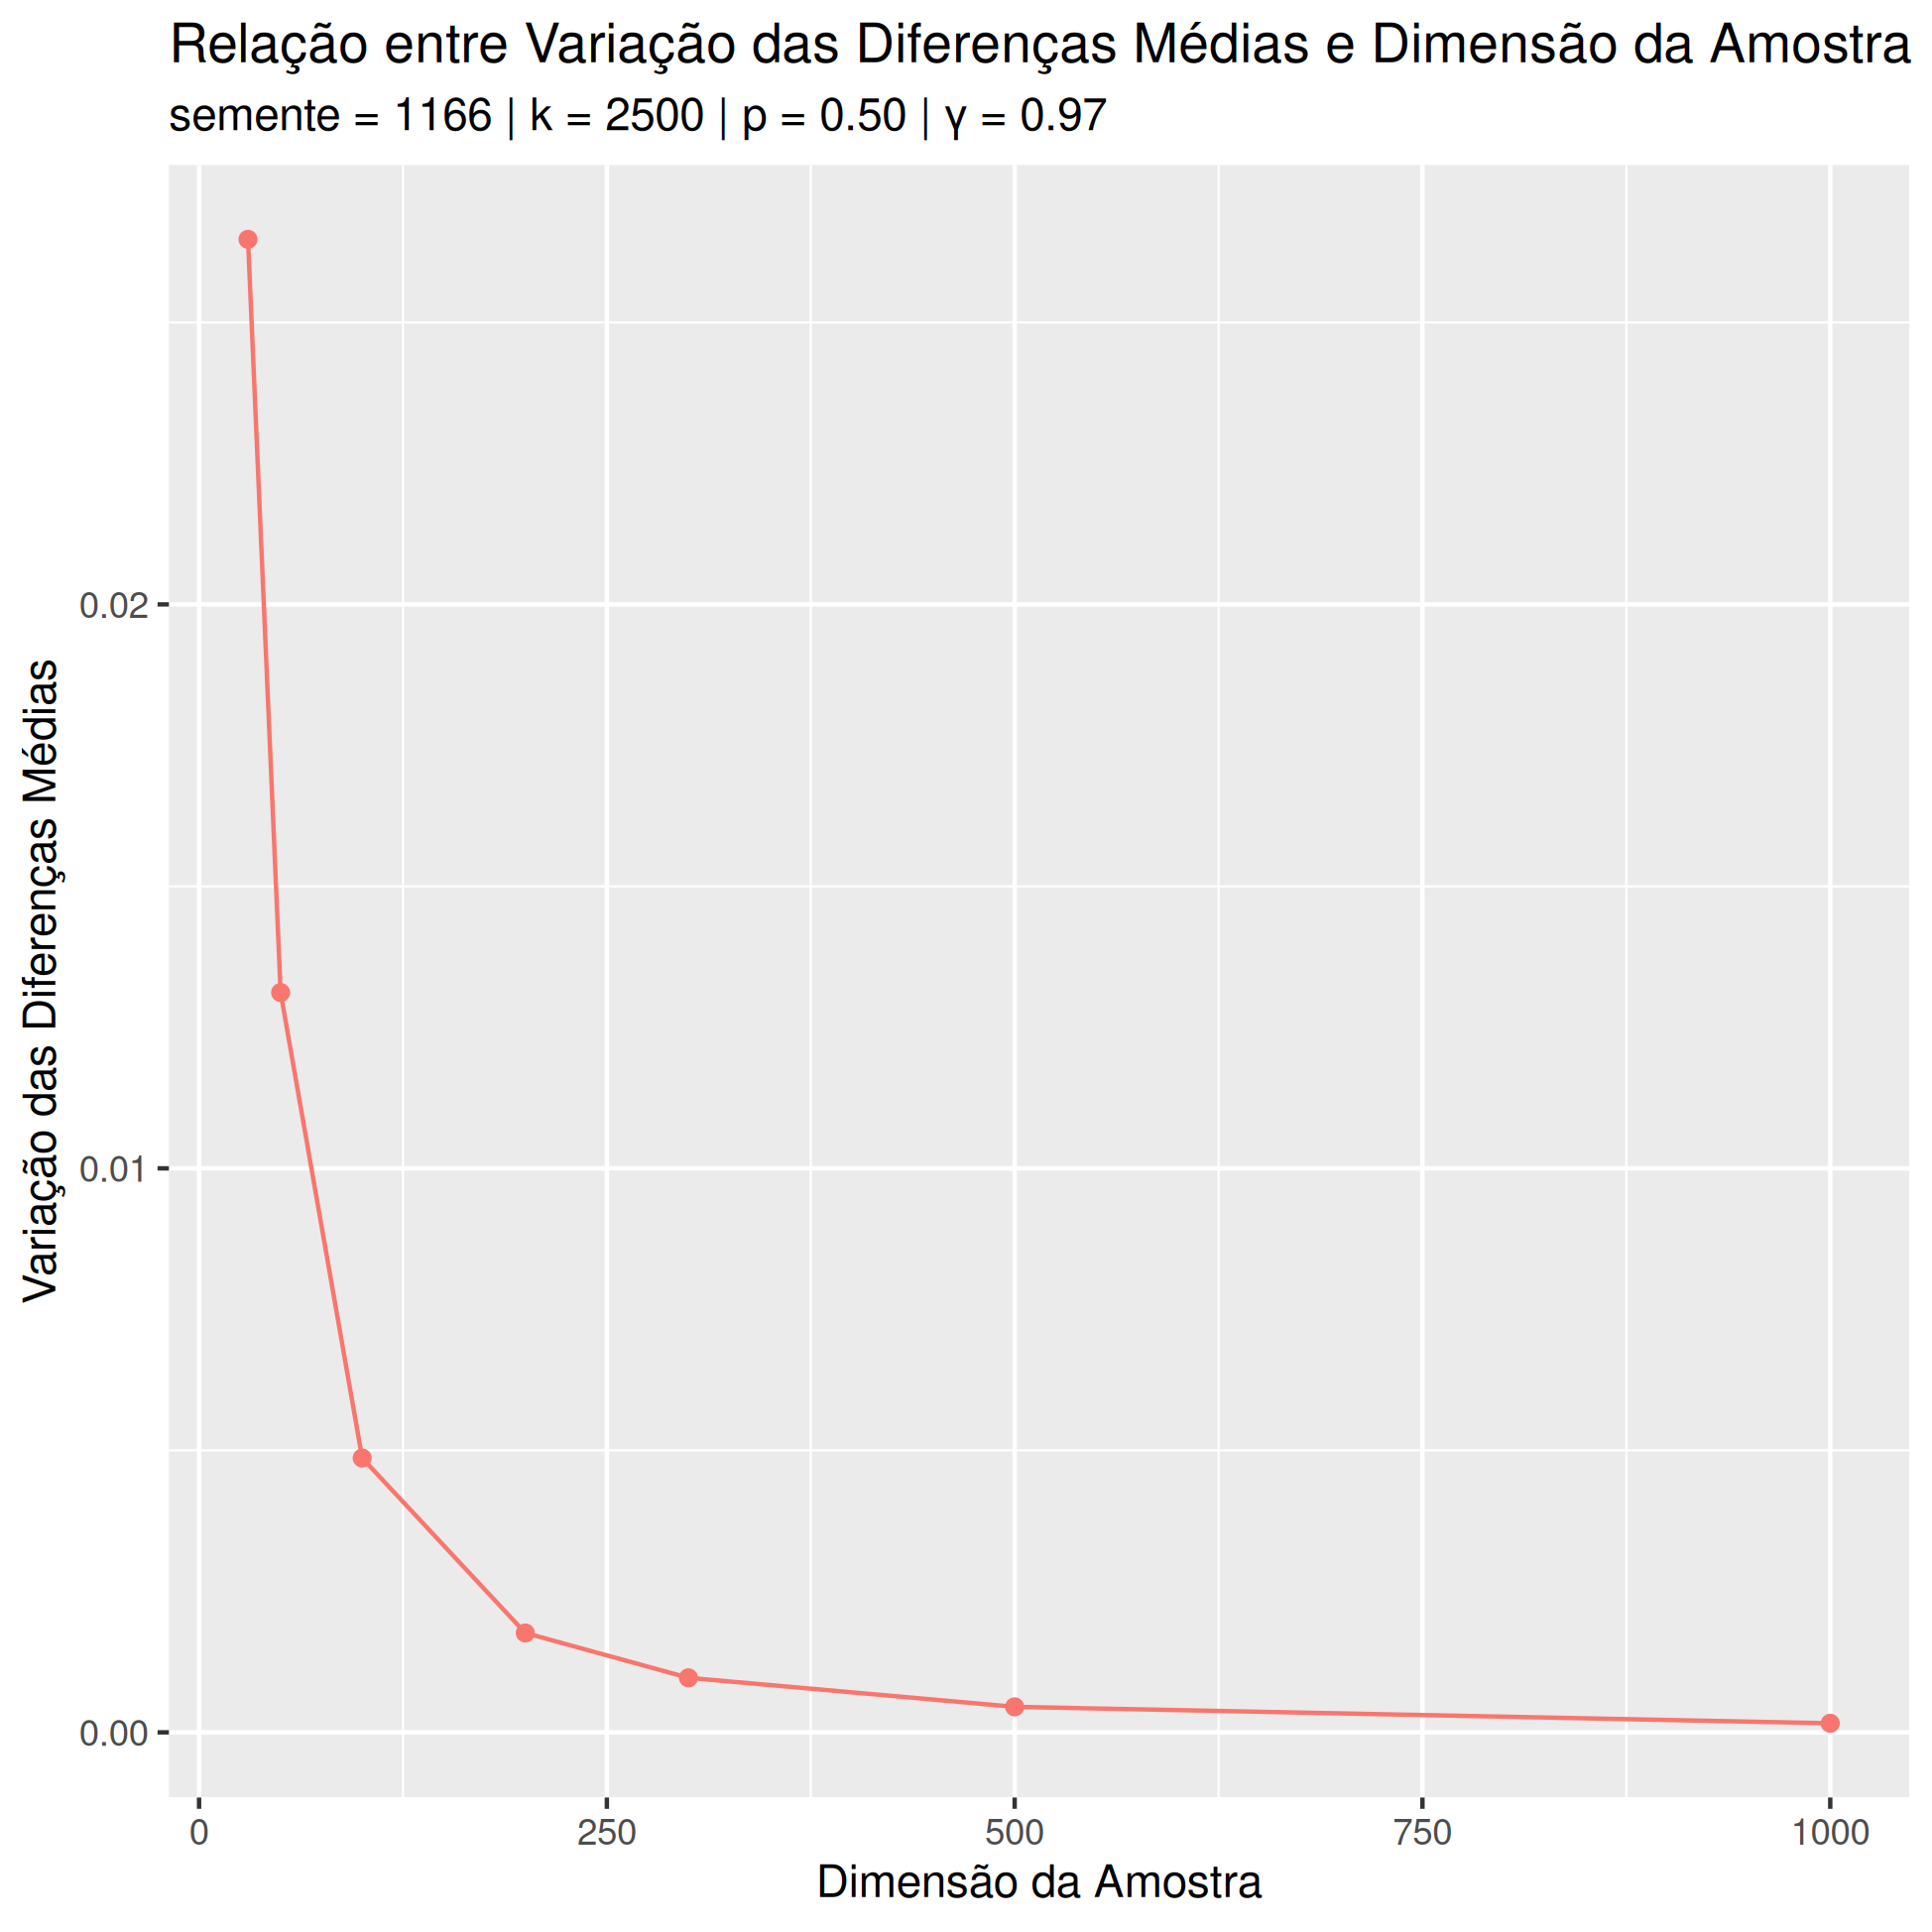
\includegraphics[width = 0.59\textwidth]{./ex09.png}
\end{wrapfigure}

% Conclusão sobre o gráfico e sobre o exercício
O gráfico obtido permite concluir que a relação entre as duas variáveis em causa é inversamente proporcional.
Deste modo, à medida que o tamanho das \texttt{2500} amostras aumenta, os métodos 1 e 2 apresentam, em média, intervalos de confiança com uma amplitude cada vez mais próxima.

As diferenças médias foram obtidas subtraindo a amplitude do método 2 pela a do método 1 para cada amostra e posteriormente calculando a média dessas diferenças.
Assim, já que todos os valores no eixo dos \texttt{yy} são positivos, conclui-se que, em geral, para amostras de dimensões mais pequenas o método 1 é mais favorável para aproximar o parâmetro \textit{p}, pois o seu intervalo de confiança tem menor amplitude.
Porém, para amostras de dimensões maiores, ambos os métodos garantem um intervalo de confiança com amplitude semelhante.

\end{document}
